\documentclass[a4paper, 11pt]{article}%тип документа
\usepackage{siunitx}
%отступы
\usepackage[left=2cm,right=2cm,top=2cm,bottom=3cm,bindingoffset=0cm]{geometry}
\usepackage[pdftex]{lscape}
%Русский язык
\usepackage[T2A]{fontenc} %кодировка
\usepackage[utf8]{inputenc} %кодировка исходного кода
\usepackage[english,russian]{babel} %локализация и переносы

%Вставка картинок
\usepackage{wrapfig}
\usepackage{graphicx}
\graphicspath{{Images/}}
\DeclareGraphicsExtensions{.pdf,.png,.jpg}

%Математика
\usepackage{amsmath, amsfonts, amssymb, amsthm, mathtools}

%Заголовокhttps://www.overleaf.com/project/6507f5a4176b25bf05722230
\author{Акимов М.И., Кондратюк Н.А. \\ Б06-206}

\title{Отчёт о выполнении лабораторной работы  \\ \textbf{Свойства электродов.}}
\date{\\6 марта 2024 года}
\begin{document}
 \maketitle

       \section{Цели работы.}
        \begin{itemize}
             \item Исследование базовых свойств электродов, способности поляризоваться (изменять заряд) под действием внешнего напряжения. 
             \item Знакомство с факторами, определяющими свойство поляризуемости.
             \item Знакомство с принципом работы трехэлектродной схемы, требованиям к электродам и их расположению.
             \item Знакомство с понятием лимитирующей стадии электрохимической реакции и двумя принципиально разными причинами изменения потенциала электрода в условиях протекания тока – при быстрой и медленной электрохимической стадии.
             \item Получение хлорсеребряного электрода и изучение его свойств.
             \item Исследование свойств платинового электрода в условиях его поляризуемости и обратимости. Оценка ключевых параметров диффузионной и кинетической стадий электрохимических реакций.
        \end{itemize}

        \section{Задачи работы.}
        \begin{itemize}
             \item Ознакомиться с содержанием работы; разобраться с работой потенциостата и соответствующего ПО.
             \item Провести катодную и анодную поляризацию серебряного электрода в растворе хлорида калия; снять соответсвующие ВАХ. 
             \item Снять и проанализировать ВАХ поляризуемого (Pt) и неполяризуемого (Ag|AgCl) электродов. 
             \item Изучить зависимость ВАХ от концентрации и скорости перемешивания для диффузионно-лимитированного процесса на электроде. 
             \item Измерить диффузионный потенциал в растворах соляной кислоты и хлорида калия при разных концентрациях.
             \item Обработать данные, рассчитать требуемые величины.
             \item Сделать выводы о соответствии результатов реальности; сделать выводы о работе в целом; сдать и оформить отчёт о выполнении лабораторной работы.
        \end{itemize}
        \newpage
\section{Теоретическое введение.}

\subsection{Поляризуемые и неполяризуемые электроды.}
\begin{wrapfigure}{l}{0.25\textwidth}
    
\includegraphics[width=0.25\textwidth]{Images/Fig. 1.png}
    \caption{Схема Эршлера-Рэндлса. $R_\text{р}$ - сопротивление раствора; $C_\text{д.с.}$ - ёмкость ДЭС; $\Theta$ - фарадеевское сопротивление.}
\end{wrapfigure} \;
\par Поляризация электрода - изменение потенциала под действием эликтрического тока. Электрический ток
может быть связан с протеканием окислительно-восстановительного процесса (фарадеевский ток) на электроде, либо с заряжением двойного электрического слоя (ток заряжения). Для наглядного понимания этих различий существует схема Эршлера-Рэндлса (Рис. 1). 

Величина фарадеевского сопротивления $\Theta$ обусловлена величиной энергетического барьера электрохимической реакции (как энергия активации для химических реакций). Для протекания тока и преодоления этого барьера необходимо прикладывать к электроду определённую величину перенапряжения. Если же $\Theta$ велико, то весь ток идёт на заряжение ёмкости ДЭС и электрическая схема представляется в виде параллельно соединённых конденсатора и резистора. В этом идеальном случае электрод называется идеально поляризуемым. В реальности с ростом заряда и потенциала электрода ток электрохимической реакции постепенно усиливается  и начинает преобладать над током заряжения. Поэтому абсолютно идеально поляризуемых электродов нет и можно говорить лишь об интервале разности потенциалов, в котором электрод можно считать поляризуемым.

Обратной ситуацией являются идеально неполяризуемые электроды с очень низким $\Theta$. Зарядить их поверхность с помощью внешнего источника напряжения практически невозможно, так как в ответ на такую попытку возникает электрический ток, сбрасывающий «лишний» заряд, оставляя потенциал практически неизменным (изменить потенциал электрода можно только в соответствии с уравнением Нернста). Типичными представителями обратимых идеально неполяризуемых электродов являются все электроды сравнения. 

\subsection{Диффузионно-лимитированный процесс и концентрационная поляризация.}\;
\par Если кинетическая стадия реакции проходит быстро и не затруднена адсорбционными
ограничениями, то электрод будет постоянно находиться в равновесии с продуктами
электрохимической реакции и величина соответствующего тока будет определяться стадией масопереноса, в частности, диффузией.


Приэлектродный неперемешиваемый слой, в котором возникает градиент концентрации реагента называется диффузионным. Принято считать, что диффузионный слой расположен непосредственно за пределами диффузного двойного электрического слоя, где восстанавливается электронейтральность раствора. В условиях стационарной диффузии можно справедливо полагать, что концентрация линейно спадает в диффузионном слое. Иначе говоря, можно описать диффузионный ток следующим соотношением:
\begin{equation*}
    i = -nFD\frac{C^{b} - C^{s}}{\delta}
    \eqno(1)
\end{equation*}
\par Заметим, что ток может расти до предельного значения, котоое называется предельным диффузионным током:
\begin{equation*}
    i_d = -nFD\frac{C^{b}}{\delta}
    \eqno(2)
\end{equation*}
\par Связь тока и потенциала устанавливается уравнением Нернста. Отличие поверхностной концентрации от ее объемного значения обуславливает сдвиг потенциала от равновесного значения, 
\begin{wrapfigure}{l}{0.25\textwidth}
    
\includegraphics[width=0.25\textwidth]{Images/Fig. 3.png}
    \caption{ВАХ для электрода с диффузионно-лимитированными стадиями восстановления и окисления.}
\end{wrapfigure}
\par поэтому такой сдвиг называется концентрационной поляризацией и определяет величину перенапряжения:
\begin{equation*}
    \eta = \left(E_0 + \frac{RT}{nF}\ln{C^{s}}\right) - \left(E_0 + \frac{RT}{nF}\ln{C^{b}}\right) = \frac{RT}{nF}\ln{\frac{C^{s}}{C^{b}}}
    \eqno(3)
\end{equation*}
\par Используя выражение (1), (2) и (3) и выражая ток, получим уравнение для величины катодного тока:
\begin{equation*}
    i = i_d \left[ 1 - exp\left(\frac{nF\eta}{RT}\right) \right]
    \eqno(4)
\end{equation*}
\par Видно, что в области малых перенапряжений экспонента раскладывается в ряд Маклорена и зависимость принимает линейный вид.
Если же диффузионно-лимитированными являются и анодный, и катодный процесс, то анодный ток описывается аналогичным (4) уравнением, а общий вид ВАХ такого электрода представлен на Рис. 2. 

\subsection{Диффузионный потенциал.}
\begin{wrapfigure}{l}{0.25\textwidth}
    
\includegraphics[width=0.25\textwidth]{Images/Fig. 2.png}
    \caption{Два раствора разной концентрации, разделённые пористой перегородкой.}
\end{wrapfigure} \;

\par Рассмотрим ситуацию на Рис. 3. В данной ситуации некоторый электролит диссоциирует на ионы и диффундирует из раствора с большей концентрацией в раствор с меньшей. Если образующиеся ионы обладают разной подвижностью и коэффициентом диффузии, то в растворе происходит пространственное разделение зарядов и возникает электрическое поле. Следовательно, через некоторый промежуток времени скорости диффундирования сравняются и между двумя частями раствора устанавливается стационарная разность потенциалов - диффузионный потенциал $\Delta \phi$. 

Все описываемые процессы описываются следующими уравнениями:
\begin{equation*}
    \overrightarrow{j} = C\overrightarrow{u} = -CB\overrightarrow{\nabla}\Tilde{\mu} = -D\overrightarrow{\nabla}C - \frac{zeD}{k_{\text{Б}}T}\overrightarrow{\nabla}\phi
    \eqno(5)
\end{equation*}
\begin{equation*}
    j_{-} = j_{+}; \; D_{+}\frac{dC_{+}}{dx} + \frac{eD_{+}C_{+}}{k_{\text{Б}}T}\frac{d\phi}{dt} = D_{-}\frac{dC_{-}}{dx} - \frac{eD_{-}C_{-}}{k_{\text{Б}}T}\frac{d\phi}{dt}
    \eqno(6)
\end{equation*}
\begin{equation*}
    \Delta \phi = \frac{k_{\text{Б}}T}{e} \frac{D_{-}-D_{+}}{D_{-}+D_{+}} \ln{\frac{C_2}{C_1}} 
    \eqno(7)
\end{equation*}
\section{Ход работы.}
\subsection{Получение и проверка работы хлорсеребряных электродов.}

    \par В начале работы очистим серебряную проволку от старого слоя AgCl с помощью катодной поляризации. Для этого соберём трёхэлектродную схему, подключая контакты $\;$"Work"$\;$ и $\;$"Comp"$\;$ к Ag рабочему электроду, а контакты $\;$"Counter"$\;$ и $\;$"Ref"$\;$ к платиновому противоэлектроду и хлорсеребрянному электроду сравнения соответственно. Измерения проводятся в режиме линейной развёртки потенциала от 0 до -1500 мВ со скоростью 10 мВ/с. Было проведено два последовательных измерения и получены вольт-амперные кривые для каждого из них (Рис. 4). 
    \begin{figure}[h!]
	\centering{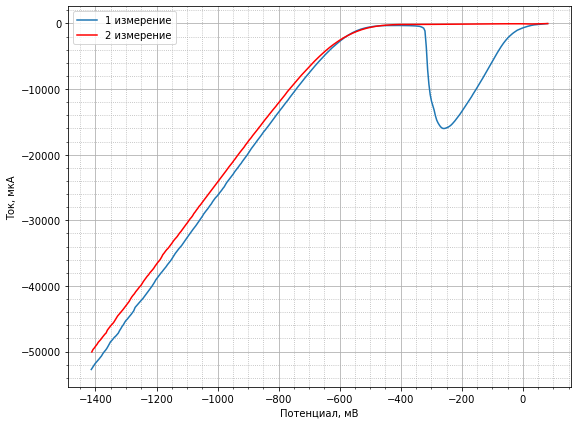
\includegraphics [scale=0.6]{Images/катодная поляризация.png}}
        \caption{График зависимости $I(E)$ при катодной поляризации.}
    \end{figure}
    
    \par Визуально наблюдали как уходил тёмный налёт (AgCl) с электрода и выделялся газ на противоэлектроде. Сопоставляя результаты с вольт-амперной кривой, получаем, что на участке от 0 до -400 мВ (образование "ямы") идёт реакция  $$AgCl + \overline{e} = Ag + Cl^-$$ На последующем линейном участке от -600 до -1400 мВ протекает реакция с выделением водорода $$2H_2O  + \overline{e} = H_2 + OH^-$$  
    
    \begin{figure}[h!]
	\centering{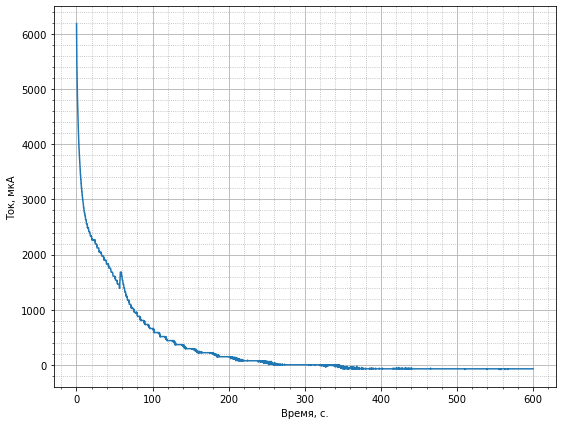
\includegraphics [scale=0.5]{Images/анодная поляризация.png}}
        \caption{График зависимости $I(t)$ при анодной поляризации.}
    \end{figure}
    \par А теперь с помощью анодной поляризации сделаем новый хлорсеребряный электрод. Для этого будем использовать потенциостатический режим на 200 мВ на 10 минут. За это время на положительно заряженном Ag электроде будет адсорбироваться $Cl^{-}$. Во время эксперимента цвет электрода постепенно становился чёрно-коричневым, а на платиновом электроде выделялся газ. Также, с потенциостата был получен график изменения потенциала со временем (Рис. 5).
    
\subsection{Поляризуемые и неполяризуемые электроды.}   \;
    \par Получим вольт-амперные характеристики следующих электродов: хлорсеребряного электрода и платинового электрода. Для этого соберём трёхэлектродную схему, подключая контакты $\,$ "Work" $\,$ и $\,$"Comp"$\,$ к исследуемым электродам, а контакты $\,$"Counter"$\,$ и $\,$"Ref"$\,$ к платиновому рабочему электроду и хлорсеребряному электроду сравнения соответственно (в ячейке находится $1$М раствор KCl). Измерения проводятся в потенциостатическом режиме работы потенциостата, на скорости развёртки около $100 \; \text{мВ}/\text{с}$ и со скоростью регистрации $13$ точек в секунду. Для наглядности опыты проводятся в несколько циклов. В результате были получены вольт-амперные кривые, приведённые на Рис. 6 и Рис. 7.

    \begin{figure}[!htb] 
        \minipage{0.5\textwidth}
            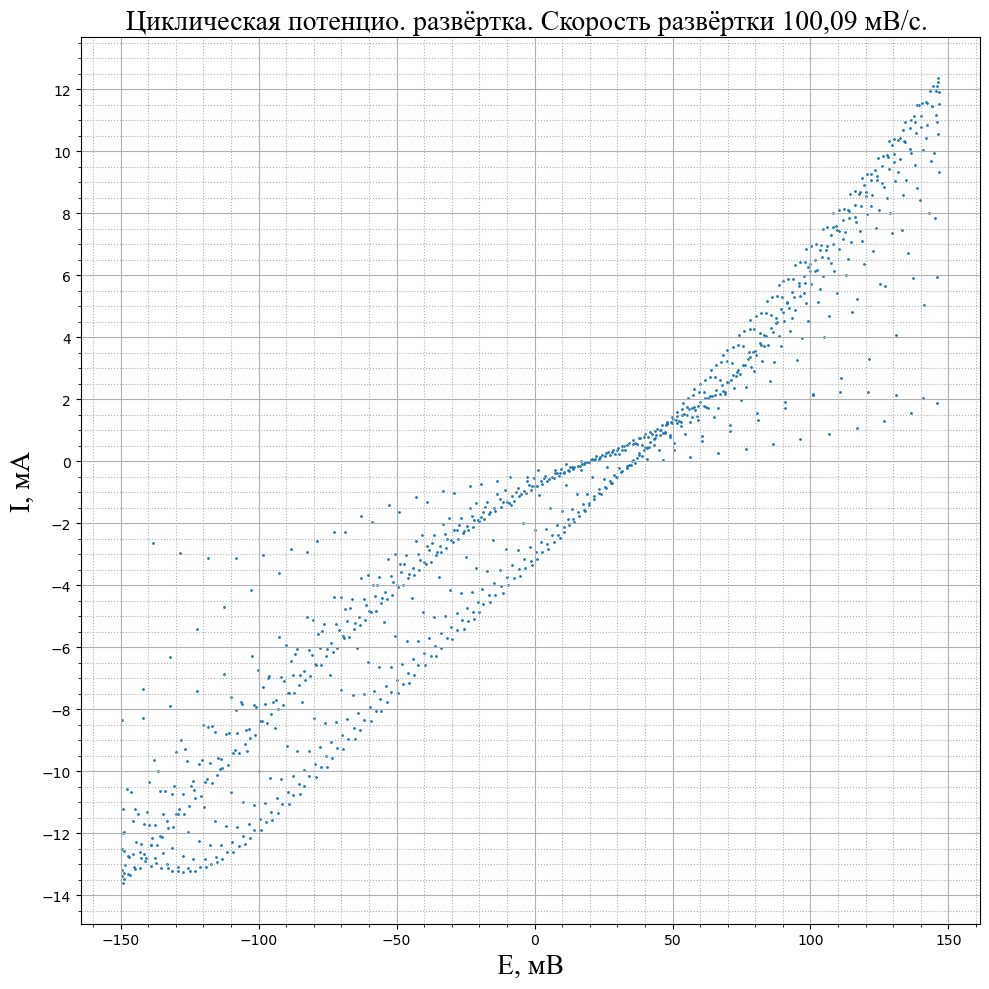
\includegraphics[width=\linewidth]{Images/Электроды.11.2.1.png}
            \caption{ВАХ Ag|AgCl - электрода.}
        \endminipage\hfill
        \minipage{0.5\textwidth}
             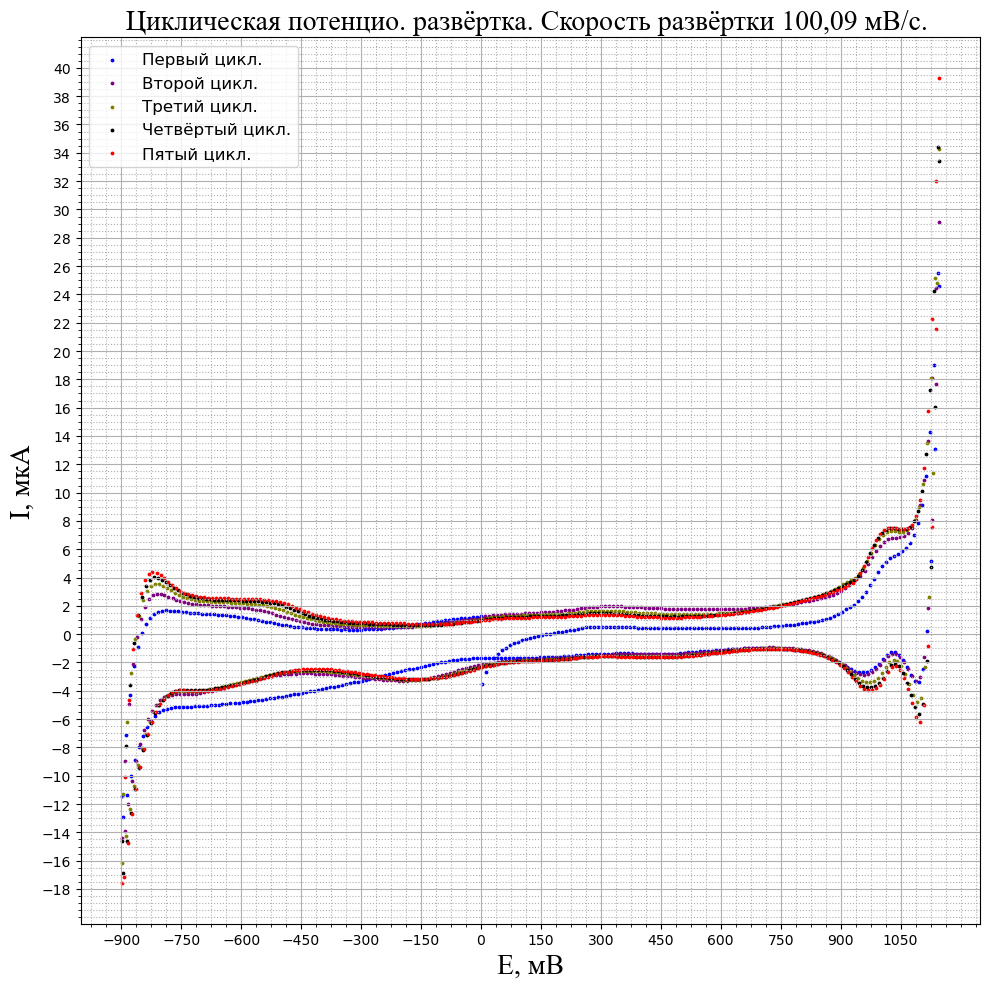
\includegraphics[width=\linewidth]{Images/Электроды.11.2.2.png}
              \caption{ВАХ Pt - электрода.}
        \endminipage
    \end{figure}

    Сопоставим экспериментальные данные с процеессами, происходящими на электродах при разных значения потенциала. 
    \begin{itemize}
        \item Ag|AgCl - электрод:
        $$I_{catod} < 0; \; AgCl + e^{-} \longrightarrow Ag + Cl^{-}$$
        $$I_{anod} > 0; \; Ag + Cl^{-} - e^{-} \longrightarrow AgCl$$
         \item Pt - электрод:
        $$I_{catod} < 0; \; 2H_{2}O + 2e^{-} \longrightarrow H_{2}\uparrow + \;2OH^{-}$$
        $$I_{anod} > 0; \;  2H_{2}O - 2e^{-}\longrightarrow O_{2}\uparrow + \; 2H^{+}$$
    \end{itemize}

    Кроме прочего, на ВАХ Pt - электрода, можно выделить плоский участок ([0 мВ, 750 мВ]), соответствующий области поляризации платинового электрода между двумя пиками, которые отвечают стандартным электродным потенциалам $E_{0}(H_{2}O/H_{2}) = -0,143$ В и $E_{0}(O_{2}/H_{2}O) = 0,820 $ В при $pH \approx 7$.

    По полученным вольт-амперным кривым, можно сделать вывод о том, что Ag|AgCl - электрод является неполяризуемым электродом (на всём измеряемом диапазоне), а Pt - электрод - поляризуемым (на области поляризации [-750 мВ, 750 мВ]). Это выглядит более очевидно, если поместить обе зависимости на один график (Рис. 8).

    \begin{figure}[h!]
	\centering{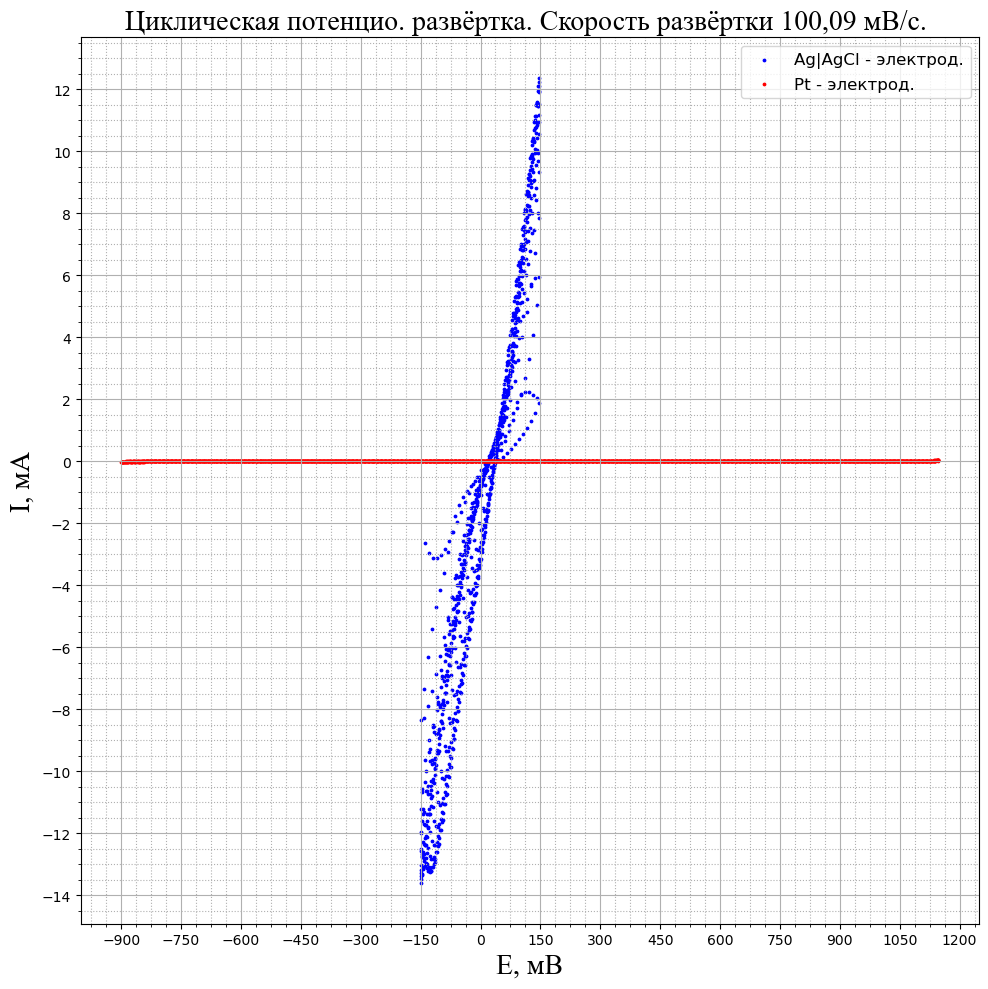
\includegraphics [scale=0.4]{Images/Электроды.11.2.3.png}}
        \caption{Совместный график ВАХ Pt - электрода и Ag|AgCl - электрода.}
    \end{figure}

\subsection{Стационарные кривые поляризации для Ox-Red электрода.}
\par Для следующего опыта будем использовать так же трёхэлектродную схему с платиновыми электродами. Однако кроме 50 мл фонового электролита (KCl) добавим по 1 мл 0.1М раствора $\mathrm{K_4[Fe(CN)_6]}$ и $\mathrm{K_3[Fe(CN)_6]}$. Зафиксируем потенциал разрыва цепи, а затем измерим кривые поляризации (катодную и анодную). Повторим измерения для разной концетрации $\mathrm{K_4[Fe(CN)_6]}$, добавляя каждый раз по 2 мл его 0.1М раствора. Полученный график изменения анодной поляризационной кривой при изменении концетрации реагента(Рис. 9) приведена ниже.

\begin{figure}[h!]
	\centering{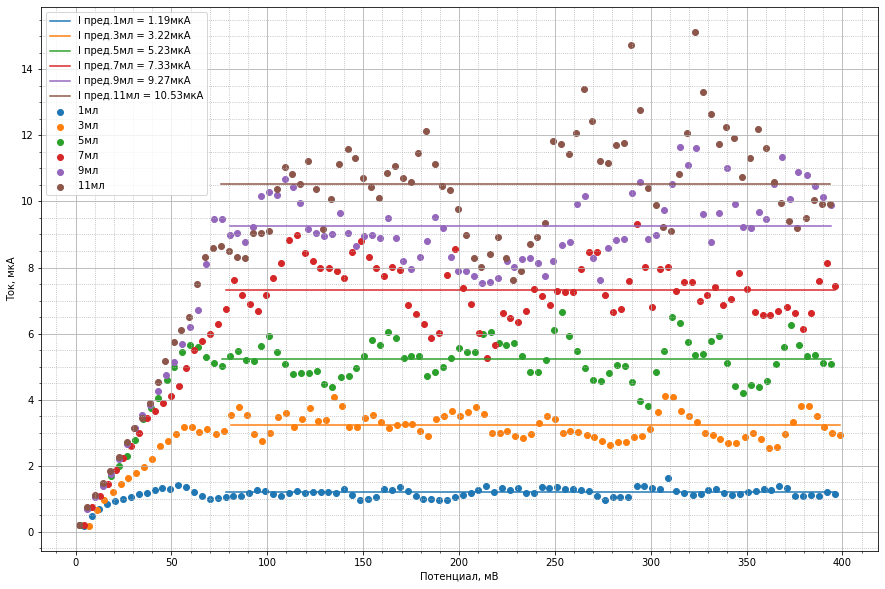
\includegraphics [scale=0.4]{Images/разные концетрации.png}}
        \caption{График зависимости $I(E)$ при последовательном добавлении $\mathrm{K_4[Fe(CN)_6]}$.}
\end{figure}
\par В электрохимической ячейке на катоде и аноде идут следующие реакции:

\[\text{Aнод}: \mathrm{Fe(CN)_6}^{4-} - \overline{e} = \mathrm{Fe(CN)_6}^{3-}\]
\[\text{Kатод}: \mathrm{Fe(CN)_6}^{3-} + \overline{e} = \mathrm{Fe(CN)_6}^{4-}\]
\par Именно поэтому мы наблюдаем изменения только для анодной ветки поляризационной кривой при добавлении $\mathrm{K_4[Fe(CN)_6]}$. 
\par Из установившейся силы тока для каждого раствора определим величину предельного диффузионного тока усреднением колеблющихся значений на плато (Рис. 9) и построим график зависимости предельного диффузионного тока от концетрации $\mathrm{K_4[Fe(CN)_6]}$ (Рис. 10).

\begin{figure}[h!]
	\centering{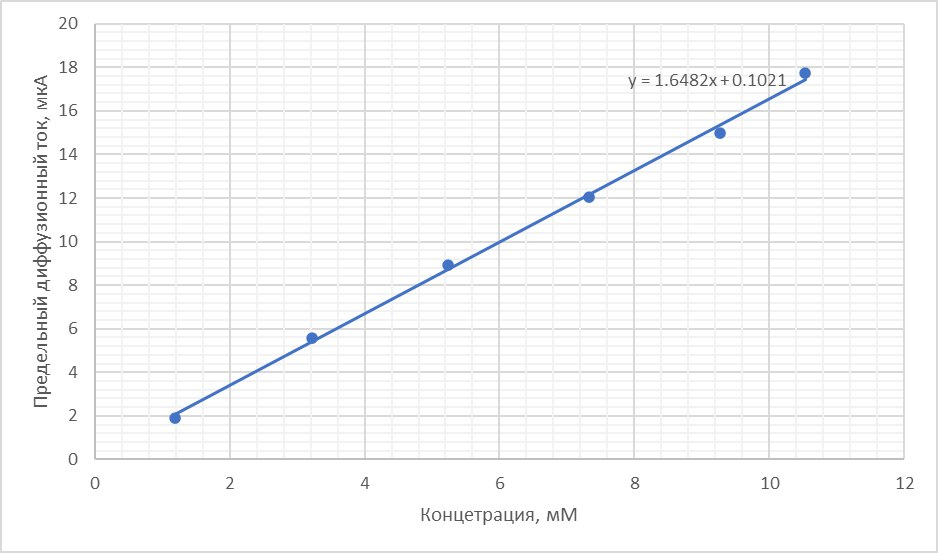
\includegraphics [scale=0.8]{Images/I(C).jpg}}
        \caption{График зависимости $I(C)$ при последовательном добавлении $\mathrm{K_4[Fe(CN)_6]}$.}
\end{figure}
\par Ток протекающей реакции можно выразить следующим образом: $I = I_d (1 - exp(\dfrac{nF\eta}{RT}))$, где предельный диффузионный ток $I_d = nFDS \dfrac{c_i}{\delta}$. Экспериментальные результаты $I_d(c_i)$ подтверждают линейную зависимость. Из коэффициента наклона прямой (Рис. 10) найдём толщину диффузионного слоя $\delta$. Из справочных данных $D = 7,4 \cdot 10^{-10} \frac{\text{м}^2}{c}\ $, отсюда найдём:

\[S = \frac{\pi d^2}{4} = 1,59 \cdot 10^{-7} \ \text{м}^2\]
\[ \delta = \frac{FDS}{k} =  6,85 \ \text{мкм}\]

\par Определим количество электронов, участвующих в реакции. При i = 0 применимо уравнение Нернста:
$$E_{Nernst} = E_0 + \frac{RT}{nF}\ln{\frac{\mathrm{K_3[Fe(CN)_6]}}{\mathrm{K_4[Fe(CN)_6]}}}$$
\par Тогда из наклона прямой графика зависимости потенциала разрыва цепи от логарифма отношений концетраций (Рис. 11) можем определить $n$.
\begin{figure}[h!]
	\centering{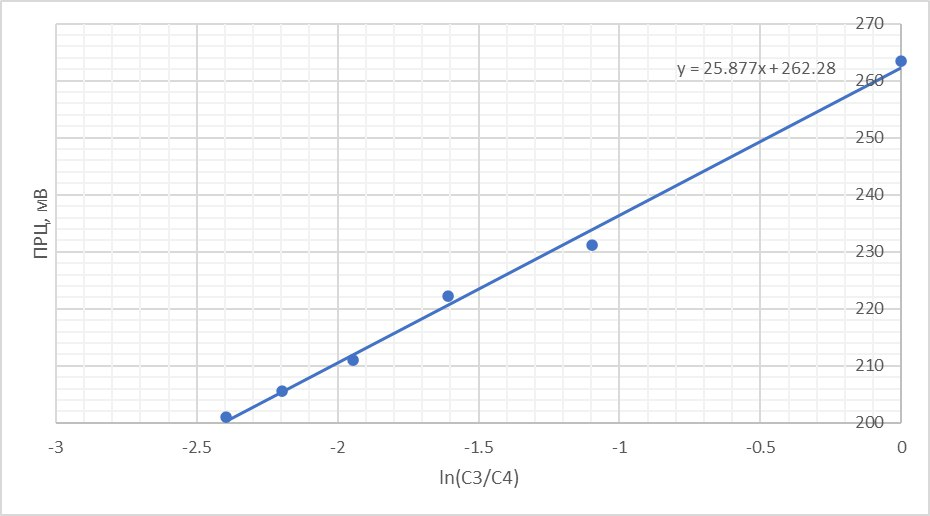
\includegraphics [scale=0.8]{Images/ПРЦ(ln).jpg}}
        \caption{График зависимости $ПРЦ(ln)$ при последовательном добавлении $\mathrm{K_4[Fe(CN)_6]}$.}
\end{figure}
\[n = \frac{RT}{kF} =  0,99 \approx 1\ \text электрон\]

\par Рассмотрим зависимость предельного диффузионного тока от скорости мешалки (Рис. 12). При более быстром перемешивании увеличивается значение предельного диффузионного тока за счёт уменьшения толщины диффузионного слоя.
\begin{figure}[h!]
	\centering{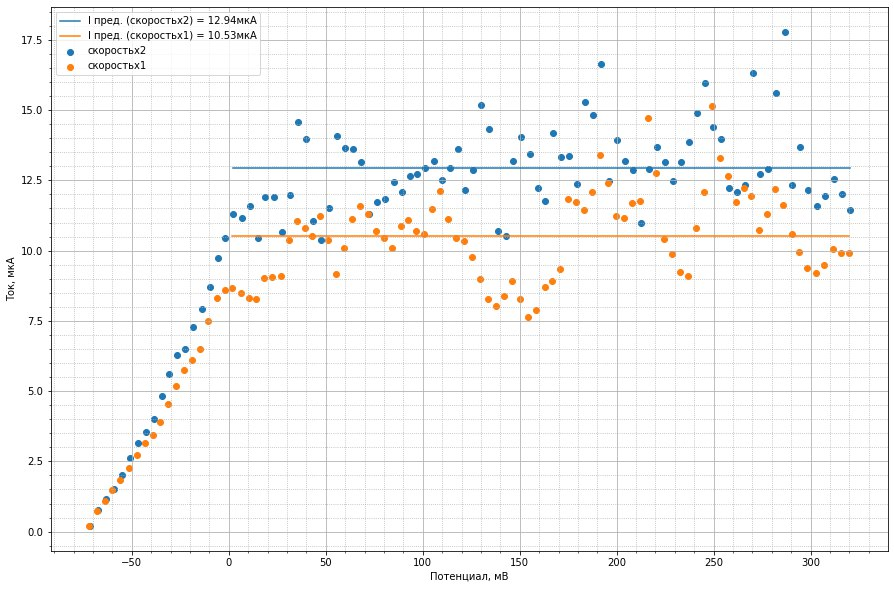
\includegraphics [scale=0.5]{Images/разные скорости.jpg}}
        \caption{График зависимости  $I(E)$ при двух скоростях перемешивания.}
\end{figure}
\newpage
\subsection{Определение диффузионного потенциала.}

Соберём двухэлектродную схему, состоящую из двух Ag|AgCl - электродов. Для этого поместим их в $0,1$М раствор HCl, подключим контакты $\;$"Counter"$\;$ и $\;$"Ref"$\;$ к одному из них, а $\;$"Comp"$\;$ и $\;$"Work"$\;$ к другому. Переведём потенциостат в режим вольтметра и будем измерять разницу потенциалов.

В результате измерения разности потенциалов двух хлорсеребряных электродов в одном и том же растворе одной и той же концентрации ожидается значение $E \approx 0$, что подтверждается экспериментально $E_{\text{эксп}} \approx -0,75$ мВ (усреднённое значение из 4627 точек, снятых за 1 мин).

Теперь перейдём к измерению диффузионного потенциала между $1$М и $0,1$М растворами HCl, соединённых электролитическим мостиком, заполненным $1$М HCl. Для этого предварительно проведём теоретический рассчёт, основываясь на формуле (7):
$$\Delta \phi = 37, 56 \; \text{мВ}$$

Так же произведём оценку Нернстовского потенциала, вносящего вклад в величину измеряемой разности потенциалов по формуле:
$$E_{Nernst} = \frac{RT}{F}\ln{\frac{C_2}{C_1}} = 58,53 \; \text{мВ}$$

В результате эксперимента вольтметр показал следующее значение разности потенциалов: $E_{\text{эксп}} = 94,00 \; \text{мВ}$. Таким образом, получаем $\Delta \phi_{\text{эксп}} = 35,47 \; \text{мВ}$, что хорошо согласуется с теоретически рассчитанным значением.

Проведём анологичный экспериммент с  растворами KCl тех же концентраций:
$$\Delta \phi = 1,11 \; \text{мВ}; \; \Delta \phi_{\text{эксп}} = 2,12 \; \text{мВ}$$

Видно, что значение согласуется с теоретическим. При этом можно сделать вывод о том, что для нивелирования диффузионного потенциала в растворах электролитов необходимо использовать электролиты, ионы которых обладают сопоставимой подвижночстью (в нашем случае это KCl), так как именно разные предельые электропроводности - подвижности - коэффициенты диффузии приводят к различным диффузионным потенциалам и на разность потенциалов между двумя электродами. 


    
\section{Выводы.}
\begin{itemize}
    \item В начале работы с помощью трёхэлектродной схемы электрохимической ячейки были рассмотрены процессы, происходящие на хлорсеребряном электроде при поляризации - катодной и анодной. В дальнейшем на приготовленном хлорсеребряном электроде исследовались свойства неполяризуемых электродов.
    \item Затем по ВАХ Pt и Ag|AgCl были проанализированы различия между поляризуемыми и неполяризуемыми электродами, соотнесены процессы, происходящие на электродах, с полученными экспериментальными зависимостями и стандарттными табличными значениями, выделена область поляризации Pt-электрода - [-750 мВ, 750 мВ].
    \item Были исследованы свойства Ox-Red электрода, а именно влияние на кривые поляризации различной концетрации реагента и скорости перемешивания. Также оценили толщину диффузного слоя: $\delta = 6,85 \text{мкм}$, что сходится с ожидаемым порядком теоретической величины, а также из уравнения Нернста было получено количество электронов, участвующих в реакции $n = 1$, что совпадает с теоретическим значением.
    \item Последней частью работы было изучение диффузионного потенциала, возникающего при опускании хлорсеребряных электродов в растворы разной концентрации (сначала HCl, затем KCl), которые были соединены электролитическим мостиком. В результате были получены значения $\Delta \phi_{HCl} = 35,47 \; \text{мВ}$ и $\Delta \phi_{KCl} = 2,12 \; \text{мВ}$, не только совпадающие с теоритически рассчитанными, но и явно отображающие большую эффективность нивелирования диффузионного потенциала при заполнении электролитического мостика раствором KCl.
\end{itemize}
\section{Приложение.}
\begin{figure}[h!]
	\centering{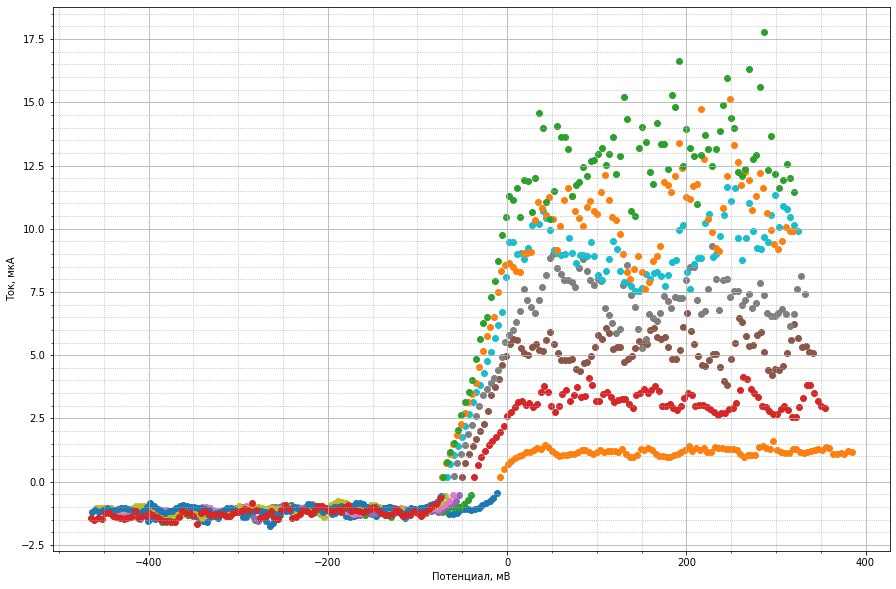
\includegraphics [scale=0.5]{Images/поляр.jpg}}
        \caption{График зависимости $I(E)$ при последовательном добавлении $\mathrm{K_4[Fe(CN)_6]}$.}
\end{figure}

\end{document}